\documentclass[12pt]{article} % Font size 12pt

\usepackage{graphicx}      % For including images
\usepackage{caption}       % For customizing captions
\usepackage{subcaption}    % For subfigures within a figure

\usepackage{fontspec}
\usepackage{polyglossia}
\usepackage{geometry}
\usepackage{hyperref} % For hyperlinks
\usepackage{enumitem}

\usepackage{tikz}
\usepackage{pgf}
\usepackage{amsmath} % for math environments and symbols
\usepackage{amssymb}
\usetikzlibrary{arrows.meta}

\usepackage{comment}
\usepackage{ifthen}
\newboolean{showexamples}
\setboolean{showexamples}{true}  % or false to hide examples
% example boxes
\usepackage{tcolorbox}
\newtcolorbox{examplebox}[1]{%
  colback=white,
  colframe=gray!30,
  title={#1},
  sharp corners,
  boxrule=0.5pt,
  coltitle=black
}

\hypersetup{
    colorlinks=true,
    linkcolor=black,   % Internal links, those generated by cross-referenced elements
    filecolor=black,  % Links to local files
    urlcolor=black,    % Links to web sites
    citecolor=black,
}

\renewenvironment{examplebox}[1]{%
  \ifthenelse{\boolean{showexamples}}%
    {\begin{tcolorbox}[colback=white, colframe=gray!30, title={#1}, sharp corners, boxrule=0.5pt, coltitle=black]}%
    {\expandafter\comment}%
}{%
  \ifthenelse{\boolean{showexamples}}%
    {\end{tcolorbox}}%
    {\expandafter\endcomment}%
}

% Set fonts
\setmainfont{CMU Serif}
\newfontfamily\greekfont{CMU Serif}

% Define \greekfonttt
\newfontfamily\greekfonttt{DejaVu Sans Mono}[Script=Greek]

% Set languages
\setdefaultlanguage{greek}
\setotherlanguage{english}

\usepackage{multicol} % For multi-column sections
% \usepackage{array}

% Set margins
\geometry{
    top=0cm,
    bottom=2cm,
    left=2cm,
    right=2cm
}

%%%%%%%%%%%%%%%%%%%%%%%%%%%%%%%%%%%%%%%%%%%%%%%%%%%%%%%%%%%%%%%%%%%%%%%%%%%%%%%%%%%%%%%%%%%%%%%%%%%%%%%%%%%%%%%%%%%%%%%%%%%%%%%%%%%%%%%%%%%%%%%%%%%%%%%%%%%%%%%%

\title{Εργασία Μέρος Β - Θεωρία Εκτίμησης και Ανίχνευσης}
\author{%
  \underline{Ομάδα 29} \\
  \begin{tabular}{ccc}
  Αριστείδης Δασκαλόπουλος & \  & Γεώργιος Ρουσομάνης \\
  arisdask@ece.auth.gr & \  & rousman@ece.auth.gr \\ 
  ΑΕΜ: 10640 & \  & ΑΕΜ: 10703
  \end{tabular}
}

\date{Ιούνιος 2025}

\begin{document}

\maketitle

\section*{Εισαγωγή}

\begin{center}
    \textit{Στόχος: Αποθορυβοποίηση πολυκαναλικών ΗΕΓ σημάτων, $\mathbf{y}[k] \in \mathbb{R}^N$, \\ που περιέχουν παρεμβολές λόγω ανοιγοκλεισίματος ματιών (blinks).}
\end{center}

\noindent\textrightarrow\ Το σήμα $y[k]$ μοντελοποιείται ως:

\vspace{-8pt}

\[
\mathbf{y}[k] = \mathbf{v}[k] + \mathbf{d}[k], \quad\text{όπου $k \in \{1, \ldots, K\}$ με $K$ το πλήθος των μετρήσεων},
\]

\vspace{-5pt}

όπου: 
\begin{itemize}[noitemsep, nolistsep]
    \item $\mathbf{v}[k]$ είναι το καθαρό δυναμικό/σήμα από την δραστηριότητα του εγκεφάλου,
    \item $\mathbf{d}[k]$ ο θόρυβος (artifact).
\end{itemize}

\vspace{+10pt}

\noindent\textrightarrow\ Για την αποθορυβοποίηση των δεδομένων με Wiener φίλτρο θα εξετάσουμε δύο μεθόδους: 
\begin{enumerate}[noitemsep, nolistsep]
    \item Στην πρώτη\textemdash offline\textemdash μέθοδο (\textit{Sections 1.*}), θα προσπαθήσουμε να εκτιμήσουμε τα καθαρά δυναμικά 
    
    \vspace{-8pt}
    
    \[
    \theta = [\mathbf{v}[0], \mathbf{v}[1], \ldots, \mathbf{v}[K-1]],
    \]
    
    \vspace{-3pt}
    
    με βάση τις τρέχουσες, παρελθοντικές και μελλοντικές τιμές των 
    $\ [\mathbf{y}[0], \ldots, \mathbf{y}[K-1]]$\textemdash \  
    \textit{Smoothing}.

    \item Στη δεύτερη\textemdash online\textemdash μέθοδο (\textit{Section 2}), θα εκτιμήσουμε καθένα από τα

    \vspace{-8pt}
    
    \[
    \theta = \mathbf{v}[m],
    \]

    \vspace{-3pt}
    
    με βάση \textit{μόνο} τις τρέχουσες και παρελθοντικές τιμές των μετρήσεων, 
    $[\mathbf{y}[0], \ldots, \mathbf{y}[k-1]]$\textemdash \textit{Filtering}.
\end{enumerate}

\vspace{+7pt}

\noindent\textrightarrow\ Για την αρχική περίπτωση, που εφαρμόζουμε την Smoothing μέθοδο, ακολουθούμε δύο προσεγγίσεις. 
Στην πρώτη\textemdash μονοκαναλική\textemdash προσέγγιση (\textit{Section 1.1}) κάθε κανάλι θα αντιμετωπίζεται ανεξάρτητα από τα υπόλοιπα, 
ενώ στην δεύτερη\textemdash πολυκαναλική\textemdash (\textit{Section 1.2}) θα λαμβάνεται υπόψιν η συσχέτιση μεταξύ των καναλιών. 
\textit{Υπενθυμίζουμε ότι ο θόρυβος που οφείλεται στο ανοιγοκλείσιμο των ματιών είναι εντονότερος στα μετωπιαία ηλεκτρόδια.}

\begin{examplebox}{Σχόλιο}
    Παρουσιάζουμε και τις δύο προσεγγίσεις αν και περιμένουμε καλύτερα αποτελέσματα στην πολυκαναλική\textemdash μιας και σε αυτήν συνυπολογίζουμε την συσχέτιση μεταξύ των καναλιών. 
    Αυτό που έχει αξία να συγκρίνουμε μεταξύ των δύο είναι το πόσο μεγάλη θα είναι η διαφορά των σφαλμάτων που εισάγει η αποθορυβοποίηση στην πράξη. 
    Από αυτήν την διαφορά θα εξάγουμε συμπεράσματα για το κατά πόσο επηρεάζει ο συνυπολογισμός της συσχέτιση μεταξύ των καναλιών την ακρίβεια των αποτελεσμάτων μας. 
\end{examplebox}

\newpage

% Set margins
\newgeometry{
    top=2cm,
    bottom=2cm,
    left=2cm,
    right=2cm
}

\section*{1.1 \ Smoothing: \textit{Μονοκαναλικό} Wiener}
\noindent Για το $i$-οστό κανάλι συμβολίζουμε ως:

\vspace{-10pt}

\begin{center}
    $\mathbf{y}_i$: τις μετρήσεις, \hspace{1cm}
    $\mathbf{v}_i$: το καθαρό δυναμικό, \hspace{1cm}
    $\mathbf{d}_i$: τον θόρυβο, 
\end{center}

\vspace{-10pt}

% \begin{itemize}[noitemsep, nolistsep]
%     \item $\mathbf{y}_i$ τις μετρήσεις, 
%     \item $\mathbf{v}_i$ το καθαρό δυναμικό, και 
%     \item $\mathbf{d}_i$ τον θόρυβο
% \end{itemize}
\noindent για τις χρονικές στιγμές $k = 0, \ldots, K - 1$.

\vspace{+10pt}

Η εκτίμηση του φίλτρου Wiener είναι:

\vspace{-10pt}

\[
\hat{\mathbf{v}}_i = \mathbf{C}_{vy}^{(i)}\left(C_{yy}^{(i)}\right)^{-1}\mathbf{y}_i, \quad i = 1,...,N,
\]

\vspace{-7pt}
\noindent με $\mathbf{C}_{vy}^{(i)}$ τον πίνακα συνδιασποράς των $\mathbf{v}_i$ \& $\mathbf{y}_i$, και $C_{yy}^{(i)}$ τον πίνακα αυτοδιασποράς του $\mathbf{y}_i$.


\vspace{+2pt}

\noindent Αν θεωρήσουμε ότι τα $\mathbf{y}_i$, $\mathbf{v}_i$, και $\mathbf{d}_i$ είναι \textbf{\textit{σήματα μηδενικής μέσης τιμής}} 
(οι χρονοσειρές των $\mathbf{y}_i$ δεν απορρίπτουν αυτήν την υπόθεση), 
και ότι τα $\mathbf{v}_i$ και $\mathbf{d}_i$ είναι μεταξύ τους ανεξάρτητα, έχουμε:

\vspace{-7pt}

\[
\begin{aligned}
    \mathbf{C}_{yy}^{(i)} &= \mathbb{E}[\mathbf{y}_i\mathbf{y}_i^T] = \mathbf{R}_{yy}^{(i)} \\
    \mathbf{C}_{vy}^{(i)} &= \mathbb{E}[\mathbf{v}_i\mathbf{y}_i^T] = 
    \mathbb{E}[\mathbf{v}_i(\mathbf{d}_i + \mathbf{v}_i)^T] = \mathbf{R}_{vv}^{(i)} \ ,
\end{aligned}
\]

\vspace{-4pt}

\noindent με $\mathbf{R}_{yy}^{(i)}, \, \mathbf{R}_{vv}^{(i)}$ τους πίνακες αυτοδιακύμανσης των χρονοσειρών
$\mathbf{y}_i, \, \mathbf{v}_i$ αντίστοιχα.

\begin{figure}[ht!]
    \centering
    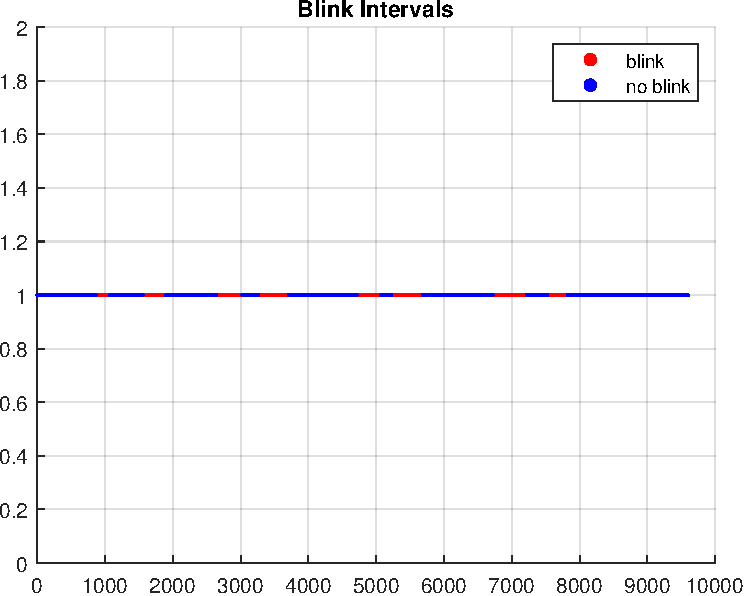
\includegraphics[width=0.5\linewidth]{plot/clean_and_noisy_intervals.pdf}
    \caption{Διαστήματα με και χωρίς θόρυβο στα δεδομένα εκπαίδευσης}
    \label{fig:clean_and_noisy_intervals}
\end{figure}

Στα δεδομένα εκπαίδευσης γνωρίζουμε εκ των προτέρων τις χρονικές στιγμές κατά τις οποίες οι μετρήσεις 
περιέχουν θόρυβο (με τις στιγμές αυτές να είναι προφανώς κοινές για όλα τα κανάλια). Επίσης, από το 
Σχήμα~\ref{fig:clean_and_noisy_intervals} παρατηρούμε ότι οι χρονικές αυτές στιγμές διαμορφώνουν διαστήματα. 
Ορίζουμε επομένως:
\[
Q = \{k = 0,...,K-1:\  \mathbf{y}[k] = \mathbf{v}[k]\} \  = \  \underset{j}{{\bigcup}} Q_j
\]

\vspace{-10pt}
\noindent με $Q_j$ το $j$-οστό διάστημα όπου $\mathbf{y}[k] = \mathbf{v}[k]$ και

\vspace{-10pt}
\[
P = \{k = 0,...,K-1:\  \mathbf{y}[k] = \mathbf{d}[k] + \mathbf{v}[k]\} \ = \ \underset{j}{{\bigcup}} P_j
\]

\vspace{-10pt}
\noindent με $P_j$ το $j$-οστό διάστημα όπου $\mathbf{y}[k] = \mathbf{d}[k] + \mathbf{v}[k]$. 

\begin{examplebox}{}
    Θα εκτιμήσουμε τον πίνακα $\mathbf{R}_{vv}^{(i)}$ από τα δεδομένα απουσίας θορύβου, δηλαδή από το σύνολο $Q$.  
    Ενώ αντίστοιχα, ο πίνακας $\mathbf{R}_{yy}^{(i)}$ θα προκύψει από τα δεδομένα παρουσίας θορύβου, δηλαδή από το σύνολο $P$.
\end{examplebox}


Θεωρώντας ότι η χρονοσειρά $\mathbf{y}_i$ είναι \textit{στάσιμη} εντός κάθε διαστήματος $Q_j$, ο πίνακας
αυτοσυσχέτισης $\mathbf{R}_{vv}^{(i,j)}$ του $i$-οστού καναλιού στο $j$-οστό διάστημα, $Q_j$, όπου απουσιάζει ο 
θόρυβος είναι:
\[
    \mathbf{R}_{vv}^{(i,j)} = 
    \begin{bmatrix}
    r_v^{(i,j)}[0] & r_v^{(i,j)}[1] & \cdots & r_v^{(i,j)}[L-1] \\
    r_v^{(i,j)}[1] & r_v^{(i,j)}[0] & \cdots & r_v^{(i,j)}[L-2] \\
    \vdots & \vdots & \ddots & \vdots \\
    r_v^{(i,j)}[L-1] & r_v^{(i,j)}[L-2] & \cdots & r_v^{(i,j)}[0]
    \end{bmatrix}
\]
όπου $r_v^{(i,j)}[\tau] = \mathbb{E}[v_i[n] v_i[n + \tau]]$, με $n, \ldots, n + \tau \in Q_j$, είναι η 
συνάρτηση αυτοσυσχέτισης του $\mathbf{v}_i$ στο διάστημα $Q_j$, και $L$ η μέγιστη υστέρηση (lag). Προφανώς, 
η μέγιστη υστέρηση που θα θέσουμε θα πρέπει να είναι μικρότερη από το μικρότερο μήκος διαστήματος με ή χωρίς θόρυβο, 
δηλαδή:
\vspace{-5pt}
\[
L \leq \min\left\{ \underset{j}{\min} |Q_j|, \; \underset{j}{\min} |P_j| \right\}, 
\]

\vspace{-4pt}
\noindent όπου ο συμβολισμός $|S|$ εκφράζει το πλήθος των στοιχείων του συνόλου $S$.

\vspace{+4pt}
Από την παραπάνω ανάλυση έχουμε ότι ο πίνακας αυτοσυσχέτισης $\mathbf{R}_{vv}^{(i)}$ μπορεί να προκύψει από τον σταθμισμένο μέσο όρο όλων των 
$\mathbf{R}_{vv}^{(i,j)}$ ως εξής:

\vspace{-4pt}
\[
\mathbf{R}_{vv}^{(i)} = \frac{1}{|Q|}\sum_{j}|Q_j|\mathbf{R}_{vv}^{(i,j)}, \quad i=1,\ldots,N
\]

\vspace{-4pt}
\noindent Εργαζόμενοι κατά ανάλογο τρόπο για τα δεδομένα παρουσία θορύβου, έχουμε:

\vspace{-5pt}
\[
\mathbf{R}_{yy}^{(i)} = \frac{1}{|P|}\sum_{j}|P_j|\mathbf{R}_{yy}^{(i,j)}, \quad i=1,\ldots,N
\]

\vspace{-4pt}
\noindent Έχοντας υπολογίσει τους δύο παραπάνω πίνακες αυτοσυσχέτισης, μπορούμε να βρούμε τον πίνακα Wiener για το $i$-οστό κανάλι:
\[
\mathbf{W}^{(i)} = \mathbf{R}_{vv}^{(i)}\left(\mathbf{R}_{yy}^{(i)}\right)^{-1} \in \mathbb{R}^{L \times L}
\]

Το φίλτρο εφαρμόζεται διαδοχικά στις μετρήσεις του εκάστοτε καναλιού, σε παράθυρα μήκους $L$, σύμφωνα με 
τη σχέση:

\vspace{-5pt}
\[
\hat{\mathbf{v}}_i[k : k + L - 1] = \mathbf{W}^{(i)} \, \mathbf{y}_i[k : k + L - 1], \quad i = 1, \ldots, N.
\]

\vspace{-4pt}
\noindent Από την πάνω σχέση είναι προφανές ότι για την εκτίμηση του $\mathbf{v}_i$ χρησιμοποιούνται κάθε φορά οι τελευταίες $L$ 
μετρήσεις του $\mathbf{y}_i$.

\begin{examplebox}{Σχόλιο}
    Είναι σημαντικό να τονίσουμε σε αυτό το σημείο ότι η συνάρτηση αυτοσυσχέτισης, και συνακόλουθα ο πίνακας 
    αυτοσυσχέτισης, λαμβάνει υπόψιν μόνο γραμμικές συσχετίσεις. Συνεπώς, το φίλτρο 
    Wiener βασίζεται στην υπόθεση της γραμμικής αυτοσυσχέτισης και 
    δεν λαμβάνει υπόψιν μη γραμμικές συσχετίσεις μεταξύ των δεδομένων της χρονοσειράς.
\end{examplebox}

Στο Σχήμα~\ref{fig:single_channel_smoothing} φαίνεται η εφαρμογή του φίλτρου στα δεδομένα εκπαίδευσης 
(αριστερά) και στα δεδομένα ελέγχου (δεξιά) για το κανάλι 1. Παρατηρούμε ότι στα δεδομένα εκπαίδευσης η
εξομάλυνση των μετρήσεων όπου υπάρχει θόρυβος (διαστήματα με μεγάλες διακυμάνσεις) είναι επιτυχής με
κόστος ωστόσο την αλοίωση της πληροφοριάς στα διαστήματα όπου δεν υπάρχει θόρυβος. Επίσης, βλέπουμε ότι
στα δεδομένα ελέγχου το φίλτρο αδυνατεί να επιτύχει την αποθορυβοποίηση του σήματος όταν παρουσιάζονται
μεγάλα \selectlanguage{english}spikes\selectlanguage{greek} του δυναμικού $> 200 V$. Αυτό εξηγείται από
το γεγονός ότι το \selectlanguage{english}Wiener\selectlanguage{greek} φίλτρο βασίζεται σε στατιστικά 
χαρακτηριστικά που υπολογίζονται από τα δεδομένα εκπαίδευσης, όπου τέτοιες ακραίες τιμές δεν εμφανίζονται. 
Τα \selectlanguage{english}spikes\selectlanguage{greek} είναι μη-γραμμικά και υψηλής 
ενέργειας γεγονότα που παραβιάζουν τις υποθέσεις στάσιμης και γραμμικής συσχέτισης πάνω στις οποίες 
βασίζεται το φίλτρο, με αποτέλεσμα την αδυναμία του να τα εξομαλύνει επαρκώς.

\begin{figure}[htbp]
    \centering
    \begin{subfigure}[b]{0.45\textwidth}
        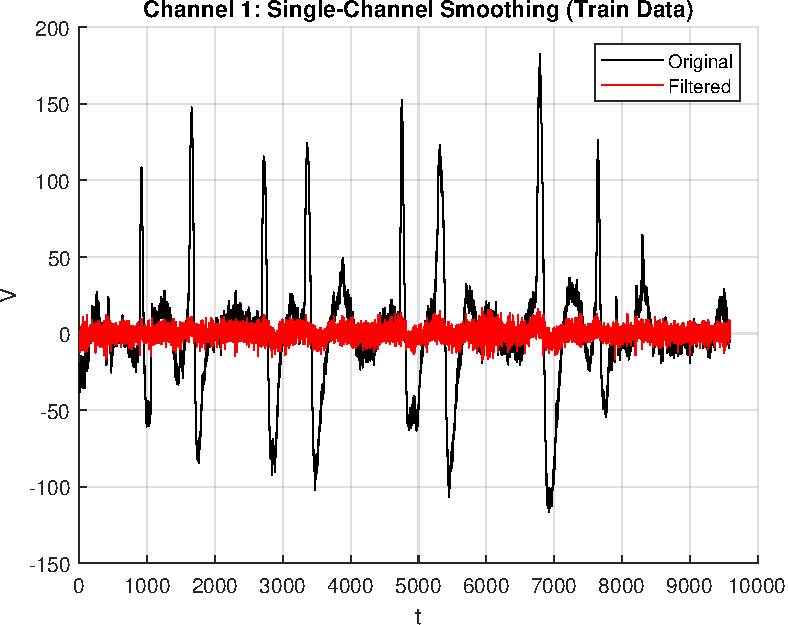
\includegraphics[width=\textwidth]{plot/single_channel_smoothing_train.pdf}
        \caption{}
        \label{fig:single_channel_smoothing_train}
    \end{subfigure}
    \hfill
    \begin{subfigure}[b]{0.45\textwidth}
        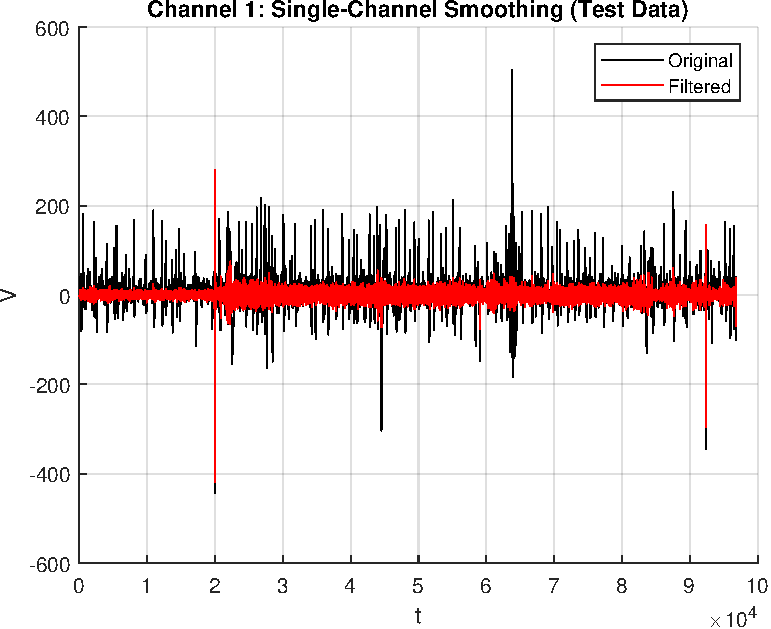
\includegraphics[width=\textwidth]{plot/single_channel_smoothing_test.pdf}
        \caption{}
        \label{fig:single_channel_smoothing_test}
    \end{subfigure}

    \caption{Εφαρμογή μονοκαναλικού \selectlanguage{english}Smoothing Wiener Filter\selectlanguage{greek} 
    στα α) δεδομένα εκπαίδευσης β) δεδομένα ελέγχου}
    \label{fig:single_channel_smoothing}
\end{figure}

\section*{1.2 \ Smoothing: \textit{Πολυκαναλικό} Wiener}
Μέχρι στιγμής, στην ανάλυσή μας εξετάζαμε κάθε κανάλι μεμονωμένα, αγνοώντας τη συσχέτιση που υπάρχει μεταξύ 
των μετρήσεών τους. Αυτό, ωστόσο, δεν είναι απολύτως ορθό, καθώς ο θόρυβος είναι εντονότερος στα μετωπιαία 
ηλεκτρόδια· επομένως, υπάρχει συσχέτιση μεταξύ των μετρήσεων διαφορετικών καναλιών. Στην παρούσα ενότητα θα 
συμπεριλάβουμε αυτές τις συσχετίσεις μεταξύ των καναλιών.

Έστω $\mathbf{Y}_t \in \mathbb{R}^{N \cdot L}$ το διάνυσμα υστέρησης, το οποίο περιέχει τις τιμές όλων των
καναλιών σε ένα παράθυρο μήκους $L$:
\[
\mathbf{Y}_t = 
\begin{bmatrix}
    \mathbf{y}_1[t:t+L-1] \\
    \mathbf{y}_2[t:t+L-1] \\
    \vdots \\
    \mathbf{y}_N[t:t+L-1] \\
\end{bmatrix}
\]
όπου $\mathbf{y}_i[t : t + L - 1] \in \mathbb{R}^L$ είναι οι μετρήσεις του $i$-οστού καναλιού.  
Επίσης, γράφουμε $\mathbf{Y}_t \equiv \mathbf{Y}_t^{(j)}$, με $t, \ldots, t + L - 1 \in P_j$.  
Χωρίς βλάβη της γενικότητας, θεωρούμε ότι το διάστημα $P_j$ ξεκινά από τη χρονική στιγμή $t = 1$.

Σχηματίζουμε τον πίνακα:
\[
\mathbf{Y}^{(j)} = 
\begin{bmatrix}
\mathbf{Y}_1^{(j)} \quad \mathbf{Y}_2^{(j)} \quad \cdots \quad \mathbf{Y}_T^{(j)}
\end{bmatrix}
\in \mathbb{R}^{N \cdot L \times T}, \quad T = |P_j| - L + 1,
\]
ή
\[
\mathbf{Y}^{(j)} = 
\begin{bmatrix}
    \mathbf{y}_1[1:L] & \mathbf{y}_1[2:L+1] & \cdots & \mathbf{y}_1[T-L+1:T] \\
    \mathbf{y}_2[1:L] & \mathbf{y}_2[2:L+1] & \cdots & \mathbf{y}_2[T-L+1:T] \\
    \vdots & \vdots & \ddots & \vdots \\
    \mathbf{y}_N[1:L] & \mathbf{y}_N[2:L+1] & \cdots & \mathbf{y}_N[T-L+1:T]
\end{bmatrix}
\]
Αν υποθέσουμε ότι $\mathbb{E}[\mathbf{Y}_t^{(j)}] = 0$, για κάθε $t = 1, \ldots, T$,  
τότε ο πίνακας συσχέτισης $\mathbf{R}_{yy}^{(j)}$ για το διάστημα $P_j$ δίνεται από:
\[
\mathbf{R}_{yy}^{(j)} = 
\frac{1}{T} \sum_{i=1}^T \mathbf{Y}_i^{(j)} \left(\mathbf{Y}_i^{(j)}\right)^{\top} = 
\frac{1}{T} \mathbf{Y}^{(j)} \cdot \left(\mathbf{Y}^{(j)}\right)^{\top}
\]
Αν, επιπλέον, οι χρονοσειρές δύο καναλιών $p$ και $q$ είναι από κοινού στάσιμες,  
δηλαδή ισχύει:
\[
\mathbb{E}[\mathbf{y}_p[k] \cdot \mathbf{y}_q[l]] = r_{pq}[k - l] \in \mathbb{R},
\]
δηλαδή η εταιροσυσχέτισή τους εξαρτάται μόνο από την υστέρηση $\tau = k - l$ και όχι από τον χρόνο, τότε:

\[
\mathbf{R}_{yy}^{(j)} =
\begin{bmatrix}
    \mathbf{R}_{11} & \mathbf{R}_{12} & \cdots & \mathbf{R}_{1N} \\
    \mathbf{R}_{21} & \mathbf{R}_{22} & \cdots & \mathbf{R}_{2N} \\
    \vdots & \vdots & \ddots & \vdots \\
    \mathbf{R}_{N1} & \mathbf{R}_{N2} & \cdots & \mathbf{R}_{NN}
\end{bmatrix}
\]
όπου $\mathbf{R}_{pq} \in \mathbb{R}^{L \times L}$ είναι ο πίνακας συνδιασποράς μεταξύ των καναλιών $p$ και 
$q$ για υστερήσεις $\tau = 0, \ldots, L - 1$. Το στοιχείο $[\mathbf{R}_{pq}]_{k, l} = r_{pq}[k - l]$ δείχνει
πόσο συσχετίζεται η τιμή του καναλιού $p$ για υστέρηση $k - 1$ με την τιμή του καναλιού $q$ για υστέρηση 
$l - 1$.

Όπως και στη μονοκαναλική προσέγγιση, ο πίνακας $\mathbf{R}_{yy}$ δίνεται από τον σταθμισμένο μέσο όρο  
των πινάκων διασποράς για όλα τα διαστήματα όπου υπάρχει θόρυβος:
\[
\mathbf{R}_{yy} = \frac{1}{|P|} \sum_j |P_j| \mathbf{R}_{yy}^{(j)}
\]

Εργαζόμενοι κατ' αντίστοιχο τρόπο στα διαστήματα $Q_j$ όπου απουσιάζει ο θόρυβος, προκύπτει ο πίνακας 
$\mathbf{R}_{vv}$.

Ο πίνακας Wiener (Wiener Smoothing Matrix) θα είναι:
\[
\mathbf{W} = \mathbf{R}_{vv}\mathbf{R}_{yy}^{-1} \in \mathbb{R}^{N \cdot L \times N \cdot L}
\]

Και εδώ το φίλτρο εφαρμόζεται διαδοχικά σε παράθυρα μήκους $L$ σύμφωνα με την σχέση:
\[
\hat{\mathbf{V}}_k = \mathbf{W} \cdot \mathbf{Y}_k
\] 
όπου $\hat{\mathbf{V}}_k \in \mathbb{R}^{N \cdot L}$ το διάνυσμα (πίνακας στήλης) με τις εκτιμήσεις του καθαρού 
σήματος όλων των καναλιών στο χρονικό παράθυρο $k,...,k+L-1$.

Στο Σχήμα~\ref{fig:multi_channel_smoothing} φαίνεται η εφαρμογή του φίλτρου στα δεδομένα εκπαίδευσης 
(αριστερά) και στα δεδομένα ελέγχου (δεξιά) για το κανάλι 1. Είναι εμφανές ότι, σε αυτή την περίπτωση, 
η απώλεια πληροφορίας στα καθαρά δεδομένα εκπαίδευσης είναι μικρότερη σε σχέση με τη μονοκαναλική προσέγγιση.  
Αυτό οφείλεται στο γεγονός ότι στην πολυκαναλική προσέγγιση λαμβάνουμε υπόψη τη συσχέτιση μεταξύ των καναλιών,  
οδηγώντας σε μικρότερες τιμές μέσου τετραγωνικού σφάλματος (άρα και RMSE).

Ωστόσο, παρατηρούμε και σε αυτή την περίπτωση ότι το φίλτρο αδυνατεί να εξομαλύνει 
\selectlanguage{english}spikes\selectlanguage{greek} του δυναμικού $ > 200 V$, καθώς, όπως έχουμε αναφέρει,
οφείλονται σε μη γραμμικές συσχετίσεις που δεν λαμβάνει υπόψη το φίλτρο 
\selectlanguage{english}Wiener\selectlanguage{greek}.

\begin{figure}[htbp]
    \centering
    \begin{subfigure}[b]{0.45\textwidth}
        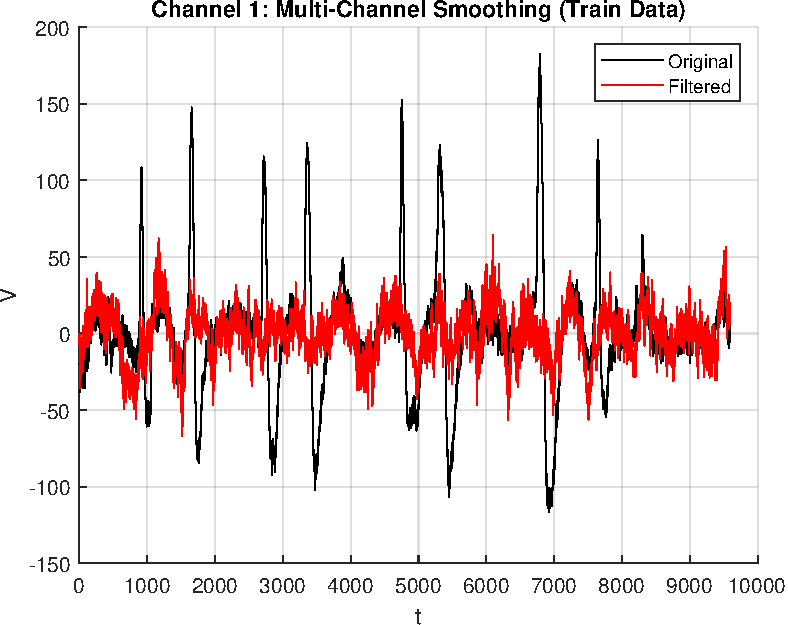
\includegraphics[width=\textwidth]{plot/multi_channel_smoothing_train.pdf}
        \caption{}
        \label{fig:multi_channel_smoothing_train}
    \end{subfigure}
    \hfill
    \begin{subfigure}[b]{0.45\textwidth}
        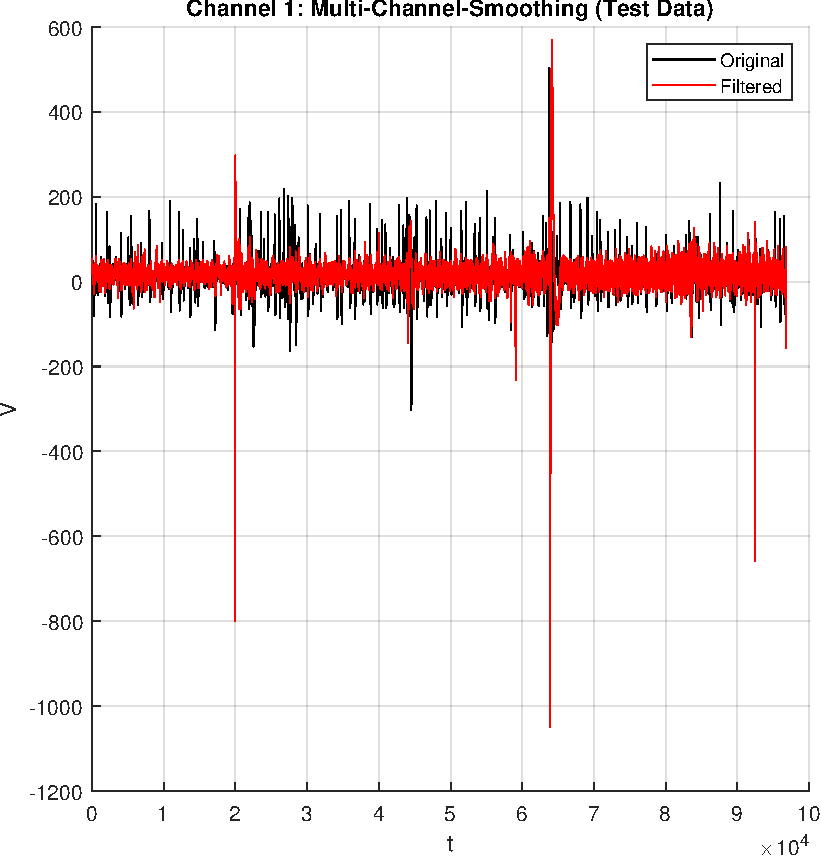
\includegraphics[width=\textwidth]{plot/multi_channel_smoothing_test.pdf}
        \caption{}
        \label{fig:multi_channel_smoothing_test}
    \end{subfigure}

    \caption{Εφαρμογή πολυκαναλικού Smoothing Wiener Filter 
    στα α) δεδομένα εκπαίδευσης β) δεδομένα ελέγχου}
    \label{fig:multi_channel_smoothing}
\end{figure}


\section*{Υλοποίηση και Σύγκριση Φίλτρων 1.1 \& 1.2}
TODO: 
1) Πρόσθεσε σημαντικά σημεία κώδικα (key parts) με μικρή εξήγηση ώστε να βγάζει νόημα. 
2) Δώσε τα αποτελέσματα των rmse και εξήγησε γτ είναι καλύτερο το Πολυκαναλικό (το έχουμε ήδη πει 2 φορές γτ, απλά πες ότι όντως φαίνεται να αξίζει πολύ περισσότερο και στην πράξη και ότι η διαφορά δεν είναι μικρή (κάθε άλλο)). 


\newpage 

\section*{2 \ Filtering: \textit{Πολυκαναλικό} Wiener}

\begin{examplebox}{Motivation}
    Με την παραπάνω ανάλυση που αφορούσε το Smoothing (και ιδιαίτερα την πολυκαναλική προσέγγιση) έχουμε ήδη καλύψει το βασικό πρόβλημα της υλοποίησης ενός Wiener φίλτρου για την αποθορυβοποίηση των δεδομένων μας από τα artifacts των blinks. 
    Από εδώ και πέρα υπάρχουν πολλές εναλλακτικές κατευθύνσεις τις οποίες θα μπορούσαμε να εξερευνήσουμε, χτίζοντας πάνω στην βασική ανάλυση που παραθέσαμε. 
    
    Αυτήν που στην συνέχεια θα δείξουμε είναι η περίπτωση που, αντί για Smoothing, επιλέγουμε να κάνουμε Filtering. 
    Ο λόγος για τον οποίο θεωρούμε πως έχει σημαντικό ενδιαφέρον είναι επειδή πρόκειται για μια online μέθοδο. 
    Άρα, αν στην πράξη θέλαμε να εφαρμόσουμε Wiener φίλτρο σε πραγματικό χρόνο (την στιγμή δηλαδή που παίρνουμε τα δεδομένα να εκτιμούμε real-time τον πίνακα $W$) τότε η μέθοδος που δείξαμε παραπάνω δεν θα μας ήταν χρήσιμη\textemdash μιας και όπως είδαμε σε αυτήν το signal sample εκτιμάται και από "μελλοντικά" data.
\end{examplebox}

`Στο Filtering πρόβλημα καλούμαστε να εκτιμήσουμε κάθε φορά το σήμα $\mathbf{v}[m]$ από το dataset των $[\mathbf{y}[0], \ldots, \mathbf{y}[m]]$. Το πρόβλημα αυτό είναι επαναλαμβανόμενο, για κάθε τιμή του m, έως ότου ολόκληρο το σήμα $\mathbf{v}[k]$, για $k = 0, 1, \ldots, K-1$ να έχει εκτιμηθεί.' (fundamentals-of-statistical-signal-processing-volume-i-estimation-theory)

Έστω $\mathbf{Y}_t \in \mathbb{R}^{N \cdot L}$ το διάνυσμα υστέρησης, το οποίο περιέχει τις τιμές όλων των
καναλιών σε ένα παράθυρο μήκους $L$:
\[
\mathbf{Y}_t = 
\begin{bmatrix}
    \mathbf{y}_1[t:t+L-1] \\
    \mathbf{y}_2[t:t+L-1] \\
    \vdots \\
    \mathbf{y}_N[t:t+L-1] \\
\end{bmatrix}
\]
όπου $\mathbf{y}_i[t : t + L - 1] \in \mathbb{R}^L$ είναι οι μετρήσεις του $i$-οστού καναλιού.  
Επίσης, γράφουμε $\mathbf{Y}_t \equiv \mathbf{Y}_t^{(j)}$, με $t, \ldots, t + L - 1 \in P_j$.  
Χωρίς βλάβη της γενικότητας, θεωρούμε ότι το διάστημα $P_j$ ξεκινά από τη χρονική στιγμή $t = 1$.

Σχηματίζουμε τον πίνακα:
\[
\mathbf{Y}^{(j)} = 
\begin{bmatrix}
\mathbf{Y}_1^{(j)} \quad \mathbf{Y}_2^{(j)} \quad \cdots \quad \mathbf{Y}_T^{(j)}
\end{bmatrix}
\in \mathbb{R}^{N \cdot L \times T}, \quad T = |P_j| - L + 1,
\]
ή
\[
\mathbf{Y}^{(j)} = 
\begin{bmatrix}
    \mathbf{y}_1[1:L] & \mathbf{y}_1[2:L+1] & \cdots & \mathbf{y}_1[T-L+1:T] \\
    \mathbf{y}_2[1:L] & \mathbf{y}_2[2:L+1] & \cdots & \mathbf{y}_2[T-L+1:T] \\
    \vdots & \vdots & \ddots & \vdots \\
    \mathbf{y}_N[1:L] & \mathbf{y}_N[2:L+1] & \cdots & \mathbf{y}_N[T-L+1:T]
\end{bmatrix}
\]
Αν υποθέσουμε ότι $\mathbb{E}[\mathbf{Y}_t^{(j)}] = 0$, για κάθε $t = 1, \ldots, T$,  
τότε ο πίνακας συσχέτισης $\mathbf{R}_{yy}^{(j)}$ για το διάστημα $P_j$ δίνεται από:
\[
\mathbf{R}_{yy}^{(j)} = 
\frac{1}{T} \sum_{i=1}^T \mathbf{Y}_i^{(j)} \left(\mathbf{Y}_i^{(j)}\right)^{\top} = 
\frac{1}{T} \mathbf{Y}^{(j)} \cdot \left(\mathbf{Y}^{(j)}\right)^{\top}
\]
Αν, επιπλέον, οι χρονοσειρές δύο καναλιών $p$ και $q$ είναι από κοινού στάσιμες,  
δηλαδή ισχύει:
\[
\mathbb{E}[\mathbf{y}_p[k] \cdot \mathbf{y}_q[l]] = r_{pq}[k - l] \in \mathbb{R},
\]
δηλαδή η εταιροσυσχέτισή τους εξαρτάται μόνο από την υστέρηση $\tau = k - l$ και όχι από τον χρόνο, τότε:

\[
\mathbf{R}_{yy}^{(j)} =
\begin{bmatrix}
    \mathbf{R}_{11} & \mathbf{R}_{12} & \cdots & \mathbf{R}_{1N} \\
    \mathbf{R}_{21} & \mathbf{R}_{22} & \cdots & \mathbf{R}_{2N} \\
    \vdots & \vdots & \ddots & \vdots \\
    \mathbf{R}_{N1} & \mathbf{R}_{N2} & \cdots & \mathbf{R}_{NN}
\end{bmatrix}
\]
όπου $\mathbf{R}_{pq} \in \mathbb{R}^{L \times L}$ είναι ο πίνακας συνδιασποράς μεταξύ των καναλιών $p$ και 
$q$ για υστερήσεις $\tau = 0, \ldots, L - 1$. Το στοιχείο $[\mathbf{R}_{pq}]_{k, l} = r_{pq}[k - l]$ δείχνει
πόσο συσχετίζεται η τιμή του καναλιού $p$ για υστέρηση $k - 1$ με την τιμή του καναλιού $q$ για υστέρηση 
$l - 1$.

Όπως και στη μονοκαναλική προσέγγιση, ο πίνακας $\mathbf{R}_{yy}$ δίνεται από τον σταθμισμένο μέσο όρο  
των πινάκων διασποράς για όλα τα διαστήματα όπου υπάρχει θόρυβος:
\[
\mathbf{R}_{yy} = \frac{1}{|P|} \sum_j |P_j| \mathbf{R}_{yy}^{(j)}
\]

Εργαζόμενοι κατ' αντίστοιχο τρόπο στα διαστήματα $Q_j$ όπου απουσιάζει ο θόρυβος, προκύπτει ο πίνακας 
$\mathbf{R}_{vv}$.

Ο πίνακας \selectlanguage{english}Wiener\selectlanguage{greek} θα είναι:
\[
\mathbf{W} = \mathbf{R}_{vv}\mathbf{R}_{yy}^{-1} \in \mathbb{R}^{N \cdot L \times N \cdot L}
\]

Και εδώ το φίλτρο εφαρμόζεται διαδοχικά σε παράθυρα μήκους $L$ σύμφωνα με την σχέση:
\[
\hat{\mathbf{V}}_k = \mathbf{W} \cdot \mathbf{Y}_k
\] 
όπου $\hat{\mathbf{V}}_k \in \mathbb{R}^{N \cdot L}$ το διάνυσμα (πίνακας στήλης) με τις εκτιμήσεις του καθαρού 
σήματος όλων των καναλιών στο χρονικό παράθυρο $k,...,k+L-1$.

Στο Σχήμα~\ref{fig:multi_channel_smoothing} φαίνεται η εφαρμογή του φίλτρου στα δεδομένα εκπαίδευσης 
(αριστερά) και στα δεδομένα ελέγχου (δεξιά) για το κανάλι 1. Είναι εμφανές ότι, σε αυτή την περίπτωση, 
η απώλεια πληροφορίας στα καθαρά δεδομένα εκπαίδευσης είναι μικρότερη σε σχέση με τη μονοκαναλική προσέγγιση.  
Αυτό οφείλεται στο γεγονός ότι στην πολυκαναλική προσέγγιση λαμβάνουμε υπόψη τη συσχέτιση μεταξύ των καναλιών,  
οδηγώντας σε μικρότερες τιμές μέσου τετραγωνικού σφάλματος (άρα και RMSE).

Ωστόσο, παρατηρούμε και σε αυτή την περίπτωση ότι το φίλτρο αδυνατεί να εξομαλύνει 
\selectlanguage{english}spikes\selectlanguage{greek} του δυναμικού $ > 200 V$, καθώς, όπως έχουμε αναφέρει,
οφείλονται σε μη γραμμικές συσχετίσεις που δεν λαμβάνει υπόψη το φίλτρο 
\selectlanguage{english}Wiener\selectlanguage{greek}.

\begin{figure}[htbp]
    \centering
    \begin{subfigure}[b]{0.45\textwidth}
        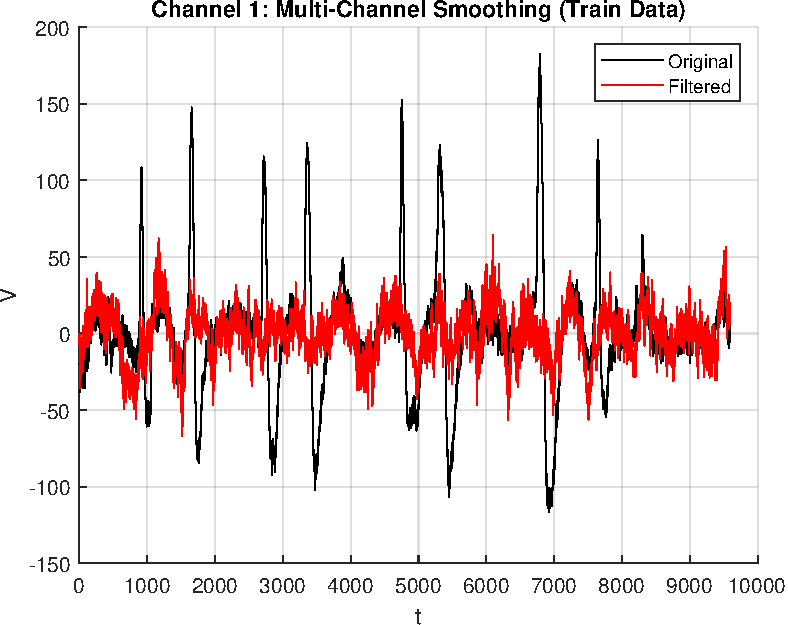
\includegraphics[width=\textwidth]{plot/multi_channel_smoothing_train.pdf}
        \caption{}
        \label{fig:multi_channel_smoothing_train}
    \end{subfigure}
    \hfill
    \begin{subfigure}[b]{0.45\textwidth}
        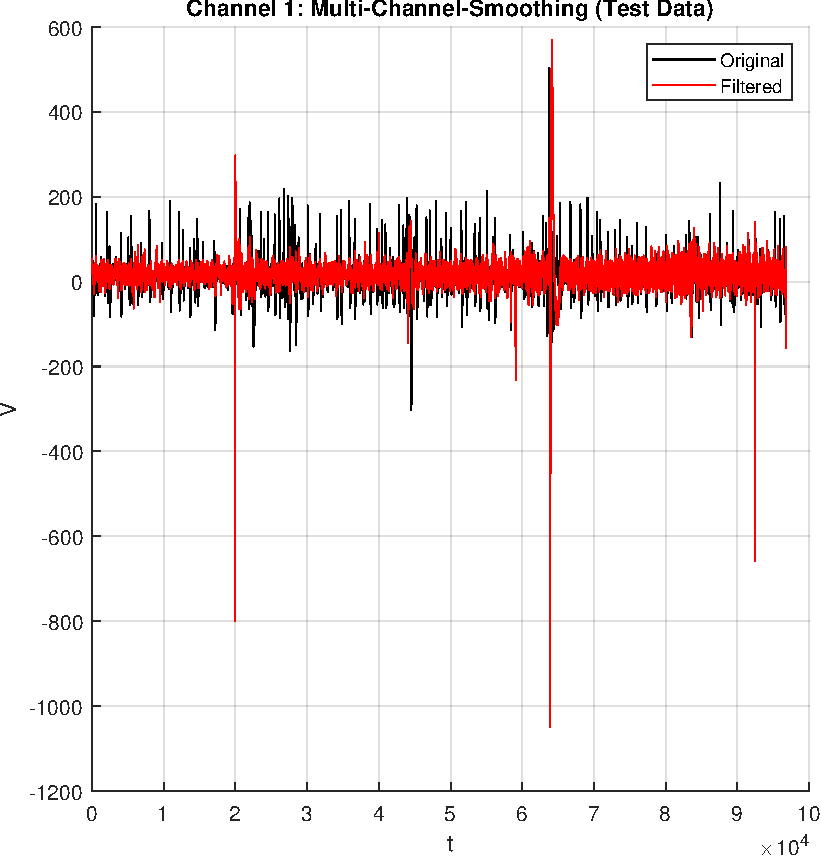
\includegraphics[width=\textwidth]{plot/multi_channel_smoothing_test.pdf}
        \caption{}
        \label{fig:multi_channel_smoothing_test}
    \end{subfigure}

    \caption{Εφαρμογή πολυκαναλικού Smoothing Wiener Filter 
    στα α) δεδομένα εκπαίδευσης β) δεδομένα ελέγχου}
    \label{fig:multi_channel_smoothing}
\end{figure}

\end{document}
